%%
\chapter{Badania własne}
\indent Proces badawczy to proces planowego, celowego wykorzystania uzyskanych informacji oraz własnej wiedzy. Celem głównym pracy jest próba stworzenia projektu świata przedstawionego w stylu graficznym low-poly. Głównym problemem jest skala. Zadecydowano więc, że projekt będzie przedstawiał trzy poziomy, w których gracz musi omijać przeszkody aby przejść na poziom wyżej.

%%
\section{Blender}
\indent Rozpoczynając pracę związaną z tworzeniem grafiki 3D, postanowiłem dowiedzieć się o możliwych programach do właśnie takich zadań. Z pośród najbardziej popularnych można wymienić Blendera, Autodesk Maya, Houdini oraz ZBrush. Jednym z kryteriów wyboru była cena zakupu programu. Oczywistym wyborem jest Blender, ponieważ jest on darmowym oprogramowaniem oraz posiada większość opcji z ww. programów. Modele wykorzystane w projekcie muszą być stworzone w stylu low-poly, oznacza to, że wymagania co do złożoności siatki obiektu pod względem topologii nie są wygórowane, wręcz muszą być zaniżone. 
%%
\section{Styl grafiki -- Low-poly}

\indent Low-poly jest określeniem siatki modelu 3D, który charakteryzuje się małą ilością wielokątów popularnie zwanych poligonami. Na przestrzeni lat, patrząc na początki gier komputerowych, dzisiejsze miano low-poly róźnie się diametralnie od swoich poprzedników z przed dwóch dekad, ze względu na o wiele większą ilość poligonów oraz technologię dzięki której tworzenie modeli 3D jest o wiele łatwiejsze, jednakże dalej odbiega od modeli które są nastawione na realizm. Wówczas obiekt zachowuje znajomom nam geometrię, jednakże nie posiada on idealnie gładkich krawędzi które odwzorcowałyby przedmiot w świecie rzeczywistym.

\begin{figure}[hbt!]
\setcaptionwidth{0.75\linewidth}
\centering
  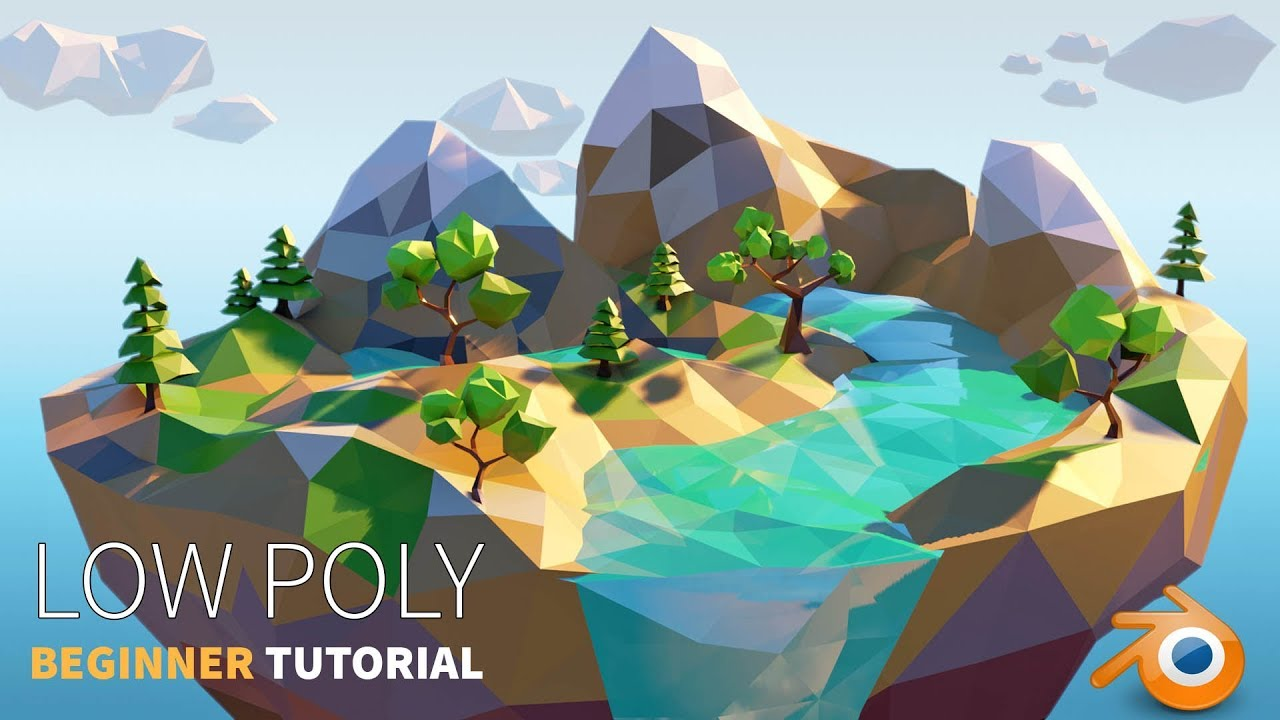
\includegraphics[width=0.75\linewidth]{lowpolytuto.jpg}
  \caption{Przykładowy render wyspy stworzonej w stylu low-poly}\label{rys_1}
  \begin{minipage}[t]{0.75\linewidth}
    \emph{Źródło: YouTube, CG Geek, Low Poly Island | Beginner | Blender 2.8 Tutorial, 2019.}
  \end{minipage}
\end{figure}

%%
\section{Unity}
\indent Istnieje wiele programów oraz silników do tworzenia gier komputerowych. Wiele dużych studiów takich jak Ubisoft, EA, CDProjektRED korzystają z własnych silników które sami napisali. Osoby, które tworzą gry w pojedynkę, korzystają z gotowych silników. Najpopularniejszymi są Unity oraz Unreal Engine. Wybierając Unity kierowałem się własnymi doświadczeniami związanymi z grami komputerowymi i programowaniem. Dużo gier, które miałem okazję zobaczyć było tworzone właśnie na silniku Unity. Unity pozwala programować w dwóch językach skryptów, C\# który jest podobny do C++, oraz JavaScript. C\# jest dla mnie bardzo intuicyjny ze względu na wielkie podobieństwo do C++ z którym miałem już doczynienia.